\chapter{Formulating Language Models as Weighted Sums}
\label{ch:weightedsum}

This chapter will show how to represent  $\ProbMKN{w_n}{w_1^{n-1}}$ and
$\ProbGLM{w_n}{w_1^{n-1}}$ as weighted sums of terms depending on $w_n$ for a
fixed history $h = w_1^{n-1}$ and an  arbitrary argument $w = w_n$.
In other words we will express the formulas given in \cref{ch:review-lm} as
equations of the following form:
\begin{equation}
  \Prob{w}{h} = \sum_{i = 1}^{N} \SumWeight_i^h \cdot \SumArg_i^h(w_n)
\end{equation}

Using this it is possible to calculate queries of type ``Noisy Channel Argmax''
(\cref{eq:noisychannel}) much more efficiently, as it is possible to perform the
(potentially expensive) calculation of $\SumWeight_i^h$ in advance.
To compute every $\Prob{w}{h}$ we now just have to calculate the
$\SumArg_i^h(w)$.

Another benefit of this representation is that it is a prerequisite of Top-$k$
joining to supply a monotone scoring function, which only depends on the
joined arguments.
Weighted sums are trivially monotone \todo{really?} and we will be able to
select our join arguments to exactly match $\SumArg_i^h$.
In addition further optimized top-$k$ joining algorithms exists, that require
weighted sum scoring functions.
However we will not use these algorithms in this work.
For a detailed discussion see \cref{ch:top-k-joining}.

In the case of Generalized Language Models our solution will also have a
considerably better computational complexity to calculate probabilities than the
na{\"\i}ve approach of just computing the formulas given in
\cref{sec:review-lm-glm}.
\begin{draft}
This will counter biggest disadvantage of GLM.
\end{draft}

We will now present the basic idea of how to transform $\Prob{w_n}{w_1^{n-1}}$
into weighted sums, that applies to both Modified Kneser-Ney Smoothing and
the Generalized Language Model as well:

Note that in all \cref{eq:mkn-high,eq:mkn-low,eq:glm-high,eq:glm-low} the
probability event $w_n$ only appears in the argument terms of
$\DiscountedCount$ or $\DiscountedCount*$.
Additionally $w_n$ occurs as arguments for $\Count$ and $\ContCountIp$ in the
lowest order \cref{eq:mkn-lowest,eq:glm-lowest}.

Our general idea is thus, to first expand recursive calls to
$\Prob(\DummyArg)$ or $\Prob*(\DummyArg)$, and second to factor
out those terms that do not depend on $w_n$ by the distributive property.
Examples of this idea are given in \cref{app:expansion}.
However they assume the history to be seen in training.
Forfeiting this assumption will add considerable complexity in the case
of Generalized Language Models.

% ------------------------------------------------------------------------------
\section{Modified Kneser-Ney Smoothing}

The first step in computing $\ProbMKN{w}{h}$ is backing off the history $h$
until $h \Skp$ is seen for the first time (\cref{eq:mkn-backoff}).
After this one pair of frequency counts $\Count(h \: w)$ and $\Count(h \Skp)$
are taken (\cref{eq:mkn-high}) and we shorten the
history by one word.
We continue this process with continuation counts $\ContCountIp(\WSkp h \: w)$
and $\ContCountIp(\WSkp h \WSkp)$ (\cref{eq:mkn-low}) until our history is
empty.
Lastly we take the frequency counts of the lowest order
(\cref{eq:mkn-lowest}).
All but the lowest order are interpolated with the next lower order via the
interpolation weight $\gamma(h)$.

Let $\SeenHistory$ be the first seen history that may be the result of backing
off given history $h$ a number of times.
The count $N$ of interpolation weights is then the number of words in
the first seen history $\SeenHistory$ plus one.
\begin{equation}
  N = \StringLength{\SeenHistory} + 1
\end{equation}

We define a helper function $\History_i(w_1^n)$ that gives the history for the
$i$th order model:
\begin{equation}
  \History_i(w_1^n) = w_i^n
\end{equation}

Building on this we can define:
\begin{align}
  \SumArg_i^h(w) &=
    \begin{dcases*}
      \Count(w)                                              & if $N = 1$ \\
      \DiscountedCount(\SeenHistory \: w)                    & if $N \neq 1 \land i = 1$ \\
      \DiscountedCount*(\WSkp \History_i(\SeenHistory) \: w) & if $N \neq 1 \land 1 < i < N$ \\
      \ContCountIp(\WSkp w)                                  & if $N \neq 1 \land i = N$
    \end{dcases*} \\
  \SumWeight_i^h &= \frac{\prod_{j = 1}^{i - 1} \gamma(\History_j(\SeenHistory))}
                        {\Count(\SeenHistory \Skp) \prod_{k = 2}^{i} \ContCountIp(\WSkp \History_k(\SeenHistory) \WSkp)}
\end{align}
\begin{equation}
  \SumWeight_i^h = \frac{1}{\Count(\SeenHistory \Skp)} \prod_{j = 2}^i \frac{\gamma(\History_{j-1}(\SeenHistory))}{\ContCountIp(\WSkp \History_j(\SeenHistory) \WSkp)}
  \vadjust{\todo{Or alternatively? Or better recursively?}}
\end{equation}

In other words, $\SumArg_i^h(w)$ is the respective frequency count that we take
on the $i$th order of interpolation.
The coefficient $\SumWeight_i^h$ weights each $\SumArg$ with the interpolation
weight $\gamma$ of all higher orders divided by the denominator frequencies of
all yet encountered orders.
\todo{Rene: wording ok?}

\todo[inline]{Do we prove that this is actually MKN?}

Specifying an algorithm to compute interpolation weights $\SumWeight_i^h$ that
minimizes frequency count lookup (using the iterative definition of
$\SumWeight_i^h$) is straightforward and given in \cref{alg:weightedsum-mkn}.

\begin{algorithm}
  \caption{\todo[inline]{Weighted Sum MKN Caption}}
  \label{alg:weightedsum-mkn}
  \begin{algorithmic}[1]
    \Require $h$
      \Comment{History for which to determinate interpolation weights}
    \Ensure $\SumWeight_i^h$
      \Comment{Array of interpolation weights}

    \LineComment{Find first seen history $\SeenHistory$}
    \State $\SeenHistory \gets h$
    \While{$\Count(\SeenHistory \Skp) = 0$}
      \State $\SeenHistory \gets \SeenHistory\text{.backoff()}$
             \todo[inline]{Better notation for backoff} 
    \EndWhile
    \State $N = \StringLength{\SeenHistory} + 1$
    \State $\SumWeight^h \gets$ new array of size $N$
    %\State
    \State $nominator \gets 1$
    \State $denominator \gets \Count(\SeenHistory \Skp)$
    \State $\SumWeight_1^h \gets \frac{1}{denominator}$
    %\State
    \State $\History \gets \SeenHistory$
    \For{$i \gets 2, N$}
      \State $nominator \gets \gamma(\History) \frac{nominator}{denominator}$
      \State $\History \gets \History\text{.backoff()}$
      \State $denominator \gets \ContCountIp(\WSkp \History \WSkp)$
      \State $\SumWeight_i^h \gets \frac{nominator}{denominator}$
    \EndFor
  \end{algorithmic}
\end{algorithm}
\begin{algorithm}
  \caption{Computing Modified Kneser-Ney sum weights}
  \begin{algorithmic}[1]
    \Require $h$
      \Comment{History for which to determinate interpolation weights}
    \Ensure $\SumWeight_i^h$
      \Comment{List of interpolation weights}

    \State $\SeenHistory \gets h$
      \Comment{Find first seen history $\SeenHistory$}
    \While{$\Count(\SeenHistory \Skp) = 0$}
      \State $\SeenHistory \gets \SeenHistory\text{.backoff()}$
             \todo[inline]{Better notation for backoff} 
    \EndWhile
    \State $N = \StringLength{\SeenHistory} + 1$
    \State $\SumWeight^h \gets$ new List of size $N$
    \State $\SumWeight_1^h \gets \frac{1}{\Count(\SeenHistory \Skp)}$
      \Comment{Set highest order weight}
    \For{$i \gets 2 \mathinner{\ldotp \ldotp} N$}
      \State $\SumWeight_i^h \gets \SumWeight_{i-1}^h \frac{\gamma(\History_{i-1}(\SeenHistory))}{\ContCountIp(\WSkp \History_i(\SeenHistory) \WSkp)}$
        \Comment{Compute lower orders using last order}
    \EndFor
    \State \todo[inline]{Replace fraction with $x^{-1}$ for better visual?}
  \end{algorithmic}
\end{algorithm}

\todo[inline]{Do we specify algorithm for MKN weighted sum (as it is rather simple)?}

% ------------------------------------------------------------------------------
\section{Generalized Language Model}

The Generalized Language Models interpolates with lower orders differently
than Modified Kneser-Ney, as described in \cref{sec:review-lm-glm}.
This section will only consider the definition of the skip operator
$\partial$ that we use in practice.
That is, $\partial_j(w_1^{n-1})$ replaces the $j$th non-skip word with a skip.
\begin{draft}
The  case of an arbitrary $\partial$ would be to complex.
\end{draft}

The case of Generalized Language Models is related to the Modified-Kneser Ney
case, although much more complex.
In a fully expanded Modified-Kneser-Ney term

\begin{draft}
Binomial Diamond.
\end{draft}

\begin{figure}
  \centering
  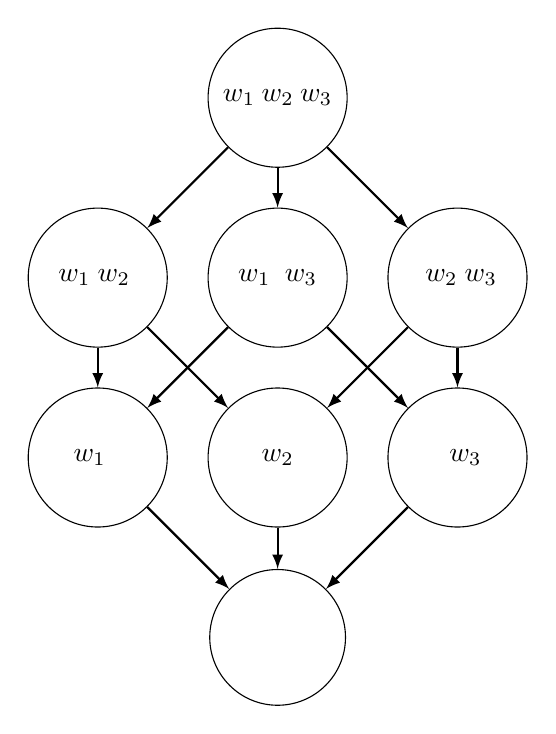
\begin{tikzpicture}[
    node distance = 6.5em,
    seq/.style = {draw, circle, align=center, text centered, text width=4.2em},
  ]
    \node [seq] (000)                {$w_1 \: w_2 \: w_3$};

    \node [seq] (010) [below of=000] {$w_1 \: \Skp \: w_3$};
    \node [seq] (001) [left  of=010] {$w_1 \: w_2 \: \Skp$};
    \node [seq] (100) [right of=010] {$\Skp \: w_2 \: w_3$};

    \node [seq] (101) [below of=010] {$\Skp \: w_2 \: \Skp$};
    \node [seq] (011) [left  of=101] {$w_1 \: \Skp \: \Skp$};
    \node [seq] (110) [right of=101] {$\Skp \: \Skp \: w_3$};

    \node [seq] (111) [below of=101] {$\Skp \: \Skp \: \Skp$};

    \path[->, >=latex, thick]
      (000) edge (001)
      (000) edge (010)
      (000) edge (100)

      (001) edge (011)
      (001) edge (101)
      (010) edge (011)
      (010) edge (110)
      (100) edge (101)
      (100) edge (110)

      (011) edge (111)
      (101) edge (111)
      (110) edge (111);
  \end{tikzpicture}
  \caption{\todo[inline]{Binomial Diamond Caption}}
\end{figure}
\begin{figure}
  \centering
  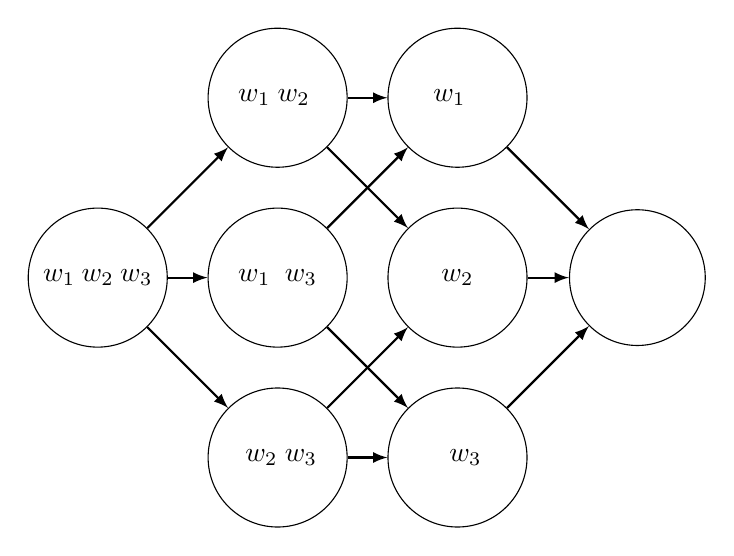
\begin{tikzpicture}[
    node distance = 6.5em,
    seq/.style = {draw, circle, align=center, text centered, text width=4.2em},
  ]
    \node [seq] (000)                {$w_1 \: w_2 \: w_3$};

    \node [seq] (010) [right of=000] {$w_1 \: \Skp \: w_3$};
    \node [seq] (001) [above of=010] {$w_1 \: w_2 \: \Skp$};
    \node [seq] (100) [below of=010] {$\Skp \: w_2 \: w_3$};

    \node [seq] (101) [right of=010] {$\Skp \: w_2 \: \Skp$};
    \node [seq] (011) [above of=101] {$w_1 \: \Skp \: \Skp$};
    \node [seq] (110) [below of=101] {$\Skp \: \Skp \: w_3$};

    \node [seq] (111) [right of=101] {$\Skp \: \Skp \: \Skp$};

    \path[->, >=latex, thick]
      (000) edge (001)
      (000) edge (010)
      (000) edge (100)

      (001) edge (011)
      (001) edge (101)
      (010) edge (011)
      (010) edge (110)
      (100) edge (101)
      (100) edge (110)

      (011) edge (111)
      (101) edge (111)
      (110) edge (111);
  \end{tikzpicture}
  \caption{\todo[inline]{Decide on graph layout}}
\end{figure}

\subsection{Bitmagic}

\subsection{Computational Complexity}
